% !TEX root =  main.tex
\newpage
\chapter{Application design} \label{ch:sw_design}
The application will be programmed in object-oriented Python, using Python processes to enable concurrent processing. 

Using processes instead of threads is necessary to utilize both cores in the intended machine, since Python employs a \emph{Global Interpreter Lock} which prevents threads within the same Python interpreter from executing concurrently. Using processes mitigates this as each process will run with its own interpreter. 

\subsection{Static structure}
structure is shown in figure \ref{figureClassDiagram} and elaborated below:

\begin{figure}[H]
    \centering
    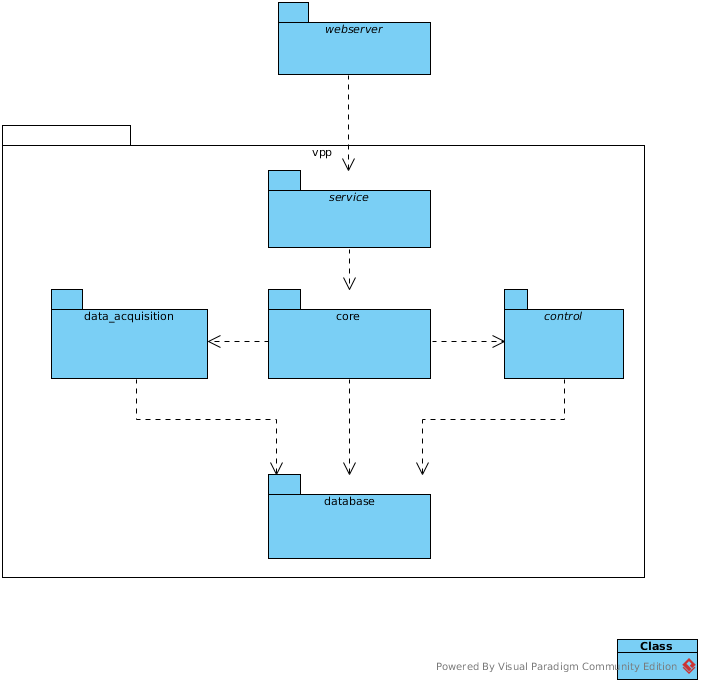
\includegraphics[width=\textwidth]{figures/class_overview}
    \caption{Class diagram. }
    \label{figureClassDiagram}
\end{figure}

The server application is roughly structured in a three-layered architecture with the \texttt{database} at lowest layer, the \texttt{core}, \texttt{control} and \texttt{data\_acquisition} packages as the middle "domain" layer and the \texttt{service} package as the top layer, providing an external interface. 

The \texttt{webserver} will access the \texttt{service} layer to provide GUI. It will be a separate application deployed on the same machine. See section \ref{subsection:webserver}.



\subsubsection{Package \texttt{vpp.core}}
This package implements the core logic of the VPP server. Classes are explained in detail below.

\begin{figure}[H]
    \centering
    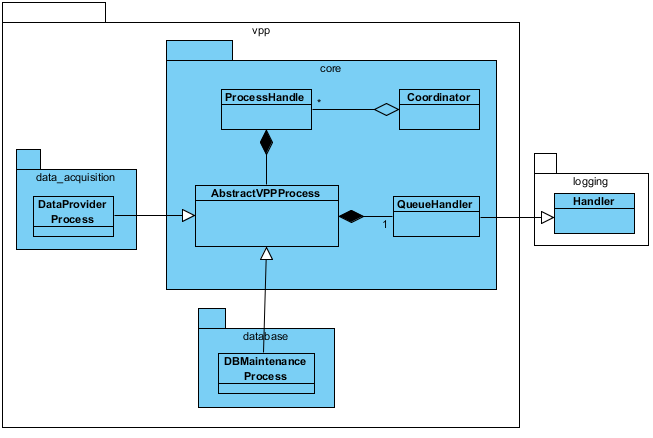
\includegraphics[width=\textwidth]{figures/class_core}
    \caption{Core}
    \label{figureClassDiagram}
\end{figure}

\texttt{Coordinator} is responsible for instantiating other classes and processes. For clarity, associations are not shown in the diagram.\\

\texttt{DataProviderProcessManager} launches the process which instantiates and manages the individual data providers that will supply measurements and predictions. \\

\texttt{ControllerManager} instantiates and keeps track of controllers for actuating physical devices. This will run in a separate process that periodically will check for and execute scheduled actions. It is expected that one process for handling all actions will be sufficient. \\

\texttt{StatusMonitor} runs a process that will poll \texttt{DataProviderManager} and \texttt{ControllerManager} for status and make this information available to the service layer.\\

\texttt{DBMonitor} runs a process that will monitor the database status. It will give information on when the last measurements were received and similar.\\

\texttt{Predictor} will run a process to create predictions based the available data.\\

\texttt{DBAccess} provides a clean interface for retrieving and posting data from and to the database. 

\subsubsection{Package \texttt{vpp.data\_acquisition}}

\begin{figure}[H]
    \centering
    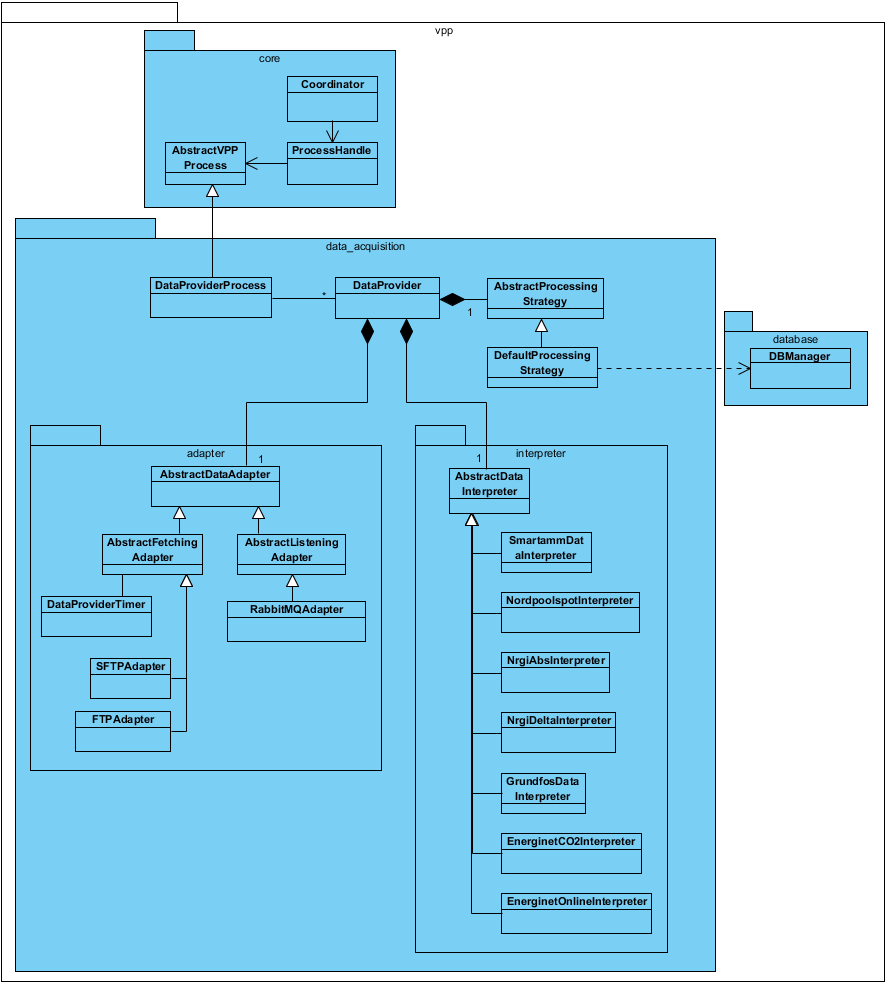
\includegraphics[width=\textwidth]{figures/class_data_acquisition}
    \caption{Data acquisition}
    \label{figureClassDiagram}
\end{figure}

This package contains the framework for connecting to various sources of measurement and prediction data. Class \texttt{DataProvider} can be instantiated in a separate thread to model a single source of data. Each \texttt{DataProvider} instance employs a suitable \texttt{DataAdapter} to communicate with for instance a message queue or a SmartAmm server.

A distinction is made between listening adapters (\texttt{AbstractListeningAdapter}), which will be activated by external events, and fetching adapters (\texttt{AbstractFetchingAdapter}) which employ an internal timer to fetch data periodically.

\subsubsection{Package \texttt{vpp.control}}
Similar to \texttt{data\_acquisition}, this package will provide a framework for communicating with the various control devices. A \texttt{Controller} can be instantiated with a suitable \texttt{ControllerAdapter} to communicate with a given device. 


\subsubsection{Package \texttt{vpp.database}}
This package contains the code that interfaces directly with the database. 

\texttt{DBMaintainer} will run maintenance on the database and implement the Rolling Window strategy.

Communication with the database could be implemented simply using SQL, or we could opt for an object-relational mapper (ORM) framework such as SQLAlchemy.


\subsection{Runtime processes}

The runtime creation of processes within the main server application is shown below:
\begin{figure}[H]
    \centering
    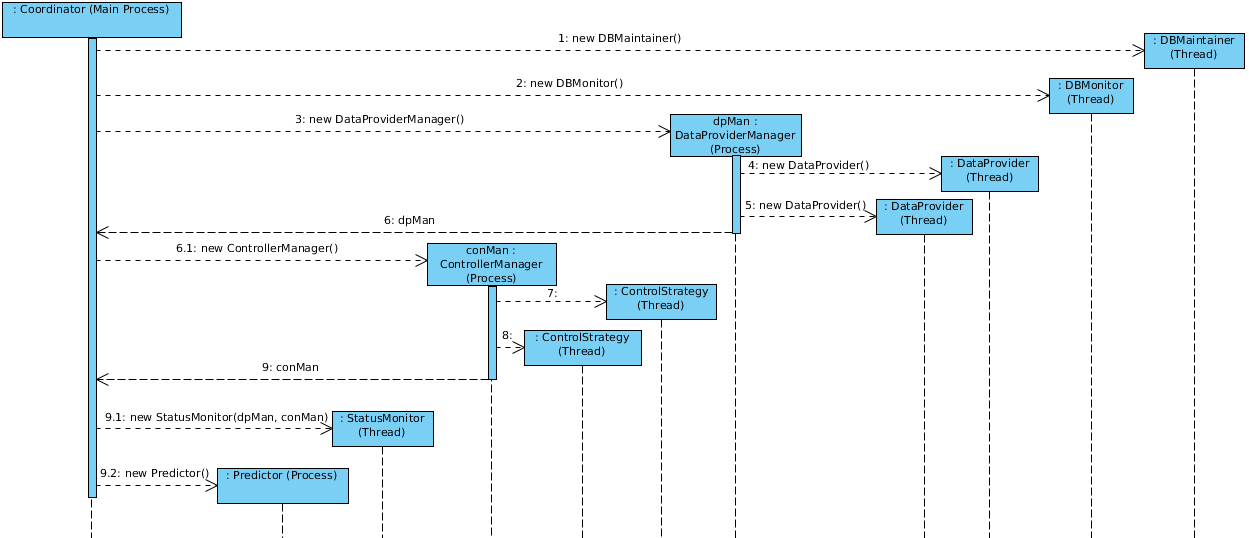
\includegraphics[width=\textwidth]{figures/seq_diagram}
    \caption{Sequence diagram of thread creation}
    \label{figureSeqDiagram}
\end{figure}
As can be seen, at least six concurrent processes will be running in addition to any \texttt{DataProviders} configured.


\subsubsection{Process communication overhead}
There is of course an overhead cost involved in running processes as opposed to threads, since processes do not have shared memory which will make communication more costly performance-wise. A balanced approach could be to group processes with frequent communication as threads within the same process, thus reducing the total number of processes form the current minimum six (plus \texttt{DataProviders}) to two or three. 

\newpage
\subsection{Data acquisition}
The execution flow when receiving measurements from a RabbitMQ is shown below:
\begin{figure}[H]
    \centering
    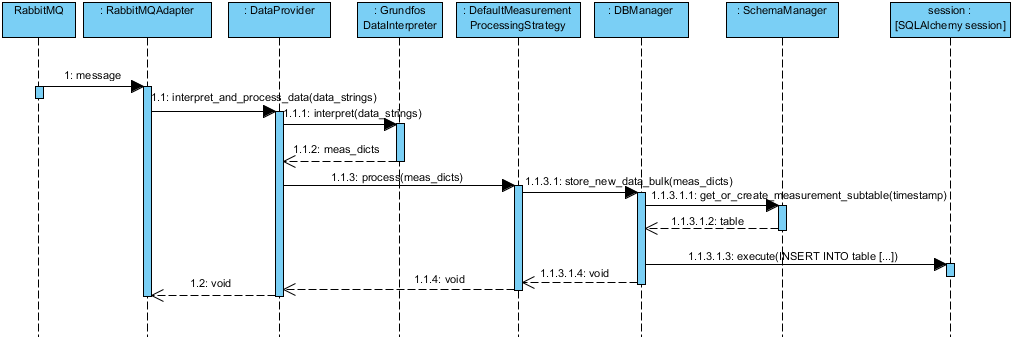
\includegraphics[width=\textwidth]{figures/data_acq_seq_diagram}
    \caption{Sequence diagram of data acquisition}
    \label{figureSeqDiagram}
\end{figure}


\subsection{Web server}\label{subsection:webserver}
We intend to provide a web interface for users to access the system. This will run in a separate web server, but in the same machine. The preliminary plan is to build the webapp using Django since this supports Python. 

The web interface could in itself grow to a rather large application with support for building configuration, device configuration, user administration, actuation interfaces and so on. This will require a substantial design and development effort. In the initial version, we plan to support only very basic interaction as proof of concept.